\documentclass[a4paper, 10pt]{article}
\usepackage[a4paper, total={5.5in, 8in}]{geometry}
\usepackage[utf8]{inputenc} % Change according your file encoding
\usepackage{graphicx}
%\usepackage[demo]{graphicx}
\usepackage{url}

\usepackage{float}
\usepackage{amsmath}
\usepackage{xcolor}
\usepackage{todonotes}

\usepackage{listings}

\definecolor{backcolour}{rgb}{0.95,0.95,0.92}

\lstdefinestyle{mystyle}{
    backgroundcolor=\color{backcolour},  
    breakatwhitespace=false,         
    basicstyle=\scriptsize,
    breaklines=true,                 
    captionpos=b,                    
    keepspaces=true,                 
    showspaces=false,                
    showstringspaces=false,
    showtabs=false,                  
    tabsize=2,
    frame=single
}



\lstset{style=mystyle}

%opening
\title{Seminar Report: Paxy}
\author{\textbf{Ignacio Encinas Rubio, Adrián Jimenez González}}
\date{\normalsize\today{}}

\begin{document}

\maketitle

%\begin{center}
  %Upload your report in PDF format.
  
  %Use this LaTeX template to format the report.
  
	%A compressed file (.tar.gz) containing all your source code files must be submitted together with this report.
%\end{center}

\section{Introduction}

The Paxy seminar consists in understanding the Paxos protocol through an Erlang implementation. First, we will develop a basic understanding of the underlying algorithm when filling the gaps in the template implementation. Later on we will build on this understanding and see the effects of different modifications such as introducing message delays, message drops, removing sorry messages and so on. Some of these modifications are specially important because they are responsible for making it impossible to guarantee a consensus in an asynchronous system.

Paxos is extensively used in production systems, so getting practical experience with it and examining how it behaves under different circumstances will prove very useful.

%\textit{Introduce in a couple of sentences the seminar and the main topic related to distributed systems it covers.}

\section{Code modifications}

   In this section we will briefly comment the code added to the template version in order to
   make the algorithm work. We will show the minimum number of lines of code possible to follow the reasoning.

  \subsection{Proposer.erl}

    \begin{minipage}{.45\textwidth}
	\begin{lstlisting}[language=erlang, caption={Template}]
	case ballot(Name, ..., ..., ..., PanelId) of  
	{ok, Value} ->
	  {Value, Round};
	abort ->
	  timer:sleep(rand:uniform(Backoff)),
	  Next = order:inc(...),
	  round(Name, (2*Backoff), ..., Proposal, Acceptors, PanelId)
	end.
	\end{lstlisting}
    \end{minipage}\hfill
    \begin{minipage}{.45\textwidth}
	\begin{lstlisting}[language=erlang, caption={Filled version}]
	case ballot(Name, Round, Proposal, Acceptors, PanelId) of
	{ok, Value} ->
	  {Value, Round};
	abort ->
	  timer:sleep(rand:uniform(Backoff)),
	  Next = order:inc(Round),
	  round(Name, (2*Backoff), Next, Proposal, Acceptors, PanelId)
	end.
	\end{lstlisting}
    \end{minipage}

    The first incomplete function is \textbf{round}. The ballot function is responsible for creating the \textit{prepare} and \textit{accept} messages from the proposer. It will need the Round in order to generate the prepare message, the Proposal to generate the accept message and the list of Acceptors for being able to send the actual messages.

    If we're not able to get our Proposal accepted we'll try again with a higher Round number after backing off for a while in order to facilitate consensus.
  

    \begin{minipage}{.45\textwidth}
	\begin{lstlisting}[language=erlang, caption={Template}]
	
  prepare(..., ...),
  Quorum = (length(...) div 2) + 1,
  MaxVoted = order:null(),
  case collect(..., ..., ..., ...) of
    {accepted, Value} ->
      accept(..., ..., ...),
      case vote(..., ...) of
        ok ->
          {ok, ...};
        abort ->
          abort
  \end{lstlisting}
    \end{minipage}\hfill
    \begin{minipage}{.45\textwidth}
	\begin{lstlisting}[language=erlang, caption={Filled version}]
	
  prepare(Round, Acceptors),
  Quorum = (length(Acceptors) div 2) + 1,
  MaxVoted = order:null(),
  case collect(Quorum, Round, MaxVoted, Proposal) of
    {accepted, Value} ->
      accept(Round, Value, Acceptors),
      case vote(Quorum, Round) of
        ok ->
          {ok, Value};
        abort ->
          abort
	\end{lstlisting}
    \end{minipage}

  For the \textbf{ballot} function we need to add \textit{Round and Acceptors} as parameters for the \textit{prepare} function. With this function we send the prepare message with the Round information to the list of Accpeptors. 

  In the next step, we need is calculate the necessary votes to achieve consensus, which is calculated as the number of Acceptors divided by 2, plus 1.

  The parameters of \textit{collect} function must be Quorum in order to know if we achieve the consensus, and Round, MaxVoted to know the maximum Round the Acceptor has promised and Proposal. In case of this function returns an accepted (also called \textit{promise} on the diagram) we call the \textit{accept} function with \textit{Round, Value, Acceptors} values as parameters to send the accept message. 

  Following that function, we call \textit{vote} fuction inside of a case statement with the Quorum and the Round, in case we recieve an ok the function will return \textit{\{ok, Value\}}.


    \begin{minipage}{.45\textwidth}
	\begin{lstlisting}[language=erlang, caption={Template}]
	
collect(N, Round, MaxVoted, Proposal) ->
  receive 
    {promise, Round, _, na} ->
      collect(..., ..., ..., ...);
    {promise, Round, Voted, Value} ->
      case order:gr(..., ...) of
        true ->
          collect(..., ..., ..., ...);
        false ->
          collect(..., ..., ..., ...)
      end;
    {promise, _, _,  _} ->
      collect(N, Round, MaxVoted, Proposal);
    {sorry, {prepare, Round}} ->
      collect(..., ..., ..., ...);
    {sorry, _} ->
      collect(N, Round, MaxVoted, Proposal)
  \end{lstlisting}
    \end{minipage}\hfill
    \begin{minipage}{.45\textwidth}
	\begin{lstlisting}[language=erlang, caption={Filled version}]
	
collect(N, Round, MaxVoted, Proposal) ->
  receive 
    {promise, Round, _, na} ->
      collect(N-1, Round, MaxVoted, Proposal);
    {promise, Round, Voted, Value} ->
      case order:gr(Voted, MaxVoted) of
        true ->
          collect(N-1, Round, Voted, Value);
        false ->
          collect(N-1, Round, MaxVoted, Proposal)
      end;
    {promise, _, _,  _} ->
      collect(N, Round, MaxVoted, Proposal);
    {sorry, {prepare, Round}} ->
      collect(N, Round, MaxVoted, Proposal);
    {sorry, _} ->
      collect(N, Round, MaxVoted, Proposal)
	\end{lstlisting}
    \end{minipage}

\todo[inline]{Terminar cuando TODO esté hecho. Preguntar al profesor en clase}

For the \textbf{collect} function, we expect to receive the reply from the acceptor to our accept. Depending on the message received our function will do:

\begin{itemize}
  \item If the message is \textit{\{promise, Round, \_, na\}}, we do recursion substracting 1 to N. Keep collecting 'support' after getting one promise.
  \item If the message is \textit{\{promise, Round, Voted, Value\}}, we are getting the promise but we need to update the maximum Voted/Proposal. That is what we do in the next case statement. We use the maximum between voted and MaxVoted for the recursion.
  \item If the message is \textit{\{sorry, \{prepare, Round\}\}}, we keep trying to get support of other Acceptors.
\end{itemize}



    \begin{minipage}{.45\textwidth}
	\begin{lstlisting}[language=erlang, caption={Template}]
	
vote(N, Round) ->
  receive
    {vote, Round} ->
      vote(..., ...);
    {vote, _} ->
      vote(N, Round);
    {sorry, {accept, Round}} ->
      vote(..., ...);
    {sorry, _} ->
      vote(N, Round)
  after ?timeout ->
    abort
  end.
  \end{lstlisting}
    \end{minipage}\hfill
    \begin{minipage}{.45\textwidth}
	\begin{lstlisting}[language=erlang, caption={Filled version}]
	
vote(N, Round) ->
  receive
    {vote, Round} ->
      vote(N-1, Round);
    {vote, _} ->
      vote(N, Round);
    {sorry, {accept, Round}} ->
      vote(N, Round);
    {sorry, _} ->
      vote(N, Round)
  after ?timeout ->
    abort
  end.
	\end{lstlisting}
    \end{minipage}

  In the \textbf{vote} function we expect to recieve a vote or sorry message from the Acceptors. In this function we define the behavior depending what we receive: 
  
  \begin{itemize}
    \item In case of receive a vote like \textit{\{vote, Round\}}, we subsctact 1 to the votes necessary for consensus (\textit{N}) to the next vote function with the same Round. 

    \item If we receive \textit{\{sorry, \{accept, Round\}\}} that means that the vote was rejected and we keep trying, so we do not substract nothing to the number of votes remaining for achieve consensus on the next vote function, passing N and Round again as parameters.
  \end{itemize}
    
    

\subsection{Acceptor.erl}


    \begin{minipage}{.45\textwidth}
	\begin{lstlisting}[language=erlang, caption={Template}]
  receive
    {prepare, Proposer, Round} ->
      case order:gr(..., ...) of
        true ->
          ... ! {promise, ..., ..., ...},               
          acceptor(Name, ..., Voted, Value, PanelId);
        false ->
          ... ! {sorry, {prepare, ...}},
          acceptor(Name, ..., Voted, Value, PanelId)
      end;
	\end{lstlisting}
    \end{minipage}\hfill
    \begin{minipage}{.45\textwidth}
	\begin{lstlisting}[language=erlang, caption={Filled version}]
  receive
    {prepare, Proposer, Round} ->
      case order:gr(Round, Promised) of
        true ->
          Proposer ! {promise, Round, Voted, Value},               
          acceptor(Name, Round, Voted, Value, PanelId);
        false ->
          Proposer ! {sorry, {prepare, Round}},
          acceptor(Name, Promised, Voted, Value, PanelId)
      end;
	\end{lstlisting}
    \end{minipage}

    The Acceptor code only has \textbf{acceptor} function to fullfil. With this function we specify the desided behavior of Acceptors. The program receives the messages of the proposers. 

    In case we receive a prepare message, we compare the Round that comes inside the message with our highest promised. 
  \begin{itemize}
    \item If the Round variable is higher we send a \textit{promise} message with the new Round, the previous \textit{Voted} round and \textit{value}. Then we update our Promised value with the Round. 
    \item Else if the value recieved in Round is lower, we send a \textit{sorry} message to the acceptor with the Round we are refusing.
  \end{itemize}


    \begin{minipage}{.45\textwidth}
	\begin{lstlisting}[language=erlang, caption={Template}]
    {accept, Proposer, Round, Proposal} ->
      case order:goe(..., ...) of
        true ->
          ... ! {vote, ...},
          case order:goe(..., ...) of
            true ->
              acceptor(Name, Promised, ..., ..., PanelId);
            false ->
              acceptor(Name, Promised, ..., ..., PanelId)
          end;                            
        false ->
          ... ! {sorry, {accept, ...}},
          acceptor(Name, Promised, Voted, Value, PanelId)
	\end{lstlisting}
    \end{minipage}\hfill
    \begin{minipage}{.45\textwidth}
	\begin{lstlisting}[language=erlang, caption={Filled version}]

    {accept, Proposer, Round, Proposal} ->
      case order:goe(Round, Promised) of
        true ->
          Proposer ! {vote, Round},
          case order:goe(Round, Voted) of
            true ->
              acceptor(Name, Promised, Round, Proposal, PanelId);
            false ->
              acceptor(Name, Promised, Round, Voted, PanelId)
          end;                            
        false ->
          Proposer ! {sorry, {accept, Round}},
          acceptor(Name, Promised, Voted, Value, PanelId)
      end;
  \end{lstlisting}
    \end{minipage}

The second type of message acceptor can receive is \textit{accept} message. In this case, we need to compare the \textit{Round} of the message with our \textit{Promised} value.

\begin{itemize}
  \item If the \textit{Round} is bigger or equal to the \textit{Promised}, we vote for the \textit{Proposal}. Then, in case the \textit{Round} is bigger or equal to \textit{Voted}, we update the highest numbered proposal, passing \textit{Round} value as \textit{Voted}. Else if it is lower, we update the the \textit{Voted} and \textit{Value} with \textit{Round} and \textit{Proposal}.
  \item If the \textit{Round} is lower than the \textit{Promised}, we send a \textit{sorry} message with the \textit{Round} value we are refusing.
\end{itemize}

\section{Experiments}
\textit{Provide evidence of the experiments you did (e.g., use screenshots) and discuss the results you got. In addition, you may provide figures or tables with experimental results of the system evaluation. For each seminar, we will provide you with some guidance on which kind of evaluation you should do.}

\subsection{Introducing delays in the promise and vote messages}
\label{sec:delays}

We have tried adding delay both to the promise and vote messages. The expected result is 
that adding delay will increase the time needed to reach consensus. As we're dealing with
random delays there is a noticeable oscillation and the runtime increase is highly volatile.
We use the same random seed for every experiment, trying to reduce the effects of pseudo-random numbers.


The increase in runtime is important but relatively controlled for small delays when compared
to the proposer timeout. The problem arises once our delay becomes so big that we start 
timing out in our proposers and we can't get work done, thus our algorithm starts taking too
much time. It is possible that it eventually achieves consensus but further examination 
is not feasable, and it wouldn't really matter as we need a somewhat reliable algorithm. 


\begin{figure}[H]
  \centering
  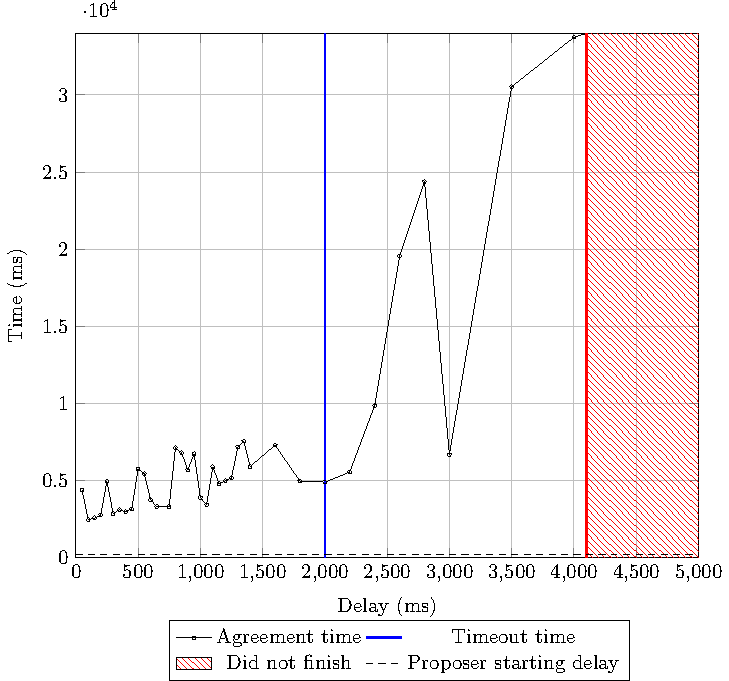
\includegraphics[width=\linewidth]{plots/exp1_timeout2000.pdf}
    \caption{Results with $\text{proposer timeout}=2000$}
\end{figure}

The number of rounds is 2 or less for almost every delay. It only increases along with the runtime spikes we see starting at $delay=2800$, where the decision starts taking 6, 9 and up to 10 rounds.
\begin{figure}[H]
  \centering
  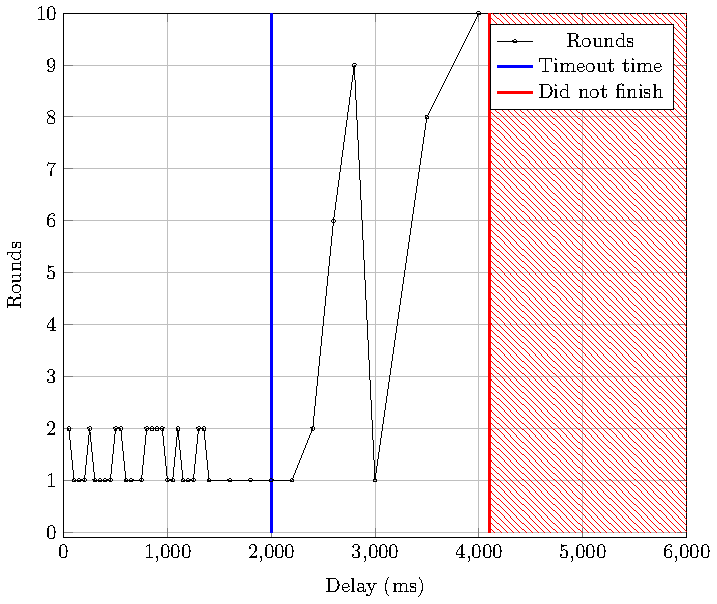
\includegraphics[width=\linewidth]{plots/roundsexp1.pdf}
    %\caption{Number of rounds needed to reach consensus respect to the delay $\text{proposer timeout}=2000$}
    \caption{Rounds needed to reach consensus w.r.t the delay\protect\footnotemark \   $\text{proposer timeout}=2000$}
\end{figure} 
\footnotetext{Actually, with respect to the mean value of the gaussian distribution it follows}


We can see a similar trend for the total number of timeouts, as shown at Figure \ref{timeouts}. The number of timeouts grows drastically once our expected delay becomes sufficiently large.

\begin{figure}[H]
  \centering
  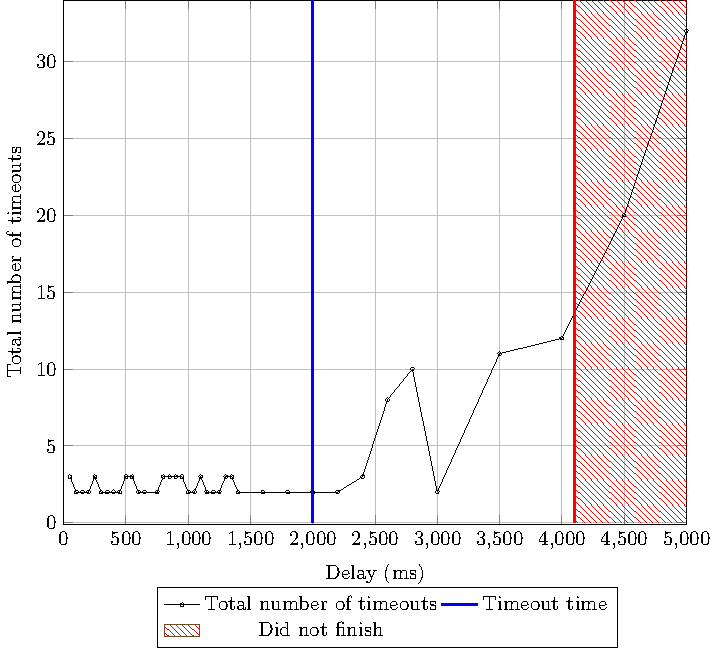
\includegraphics[width=\linewidth]{plots/timeouts.pdf}
    %\caption{Number of rounds needed to reach consensus respect to the delay $\text{proposer timeout}=2000$}
    \caption{Number of timeouts w.r.t the delay\   $\text{proposer timeout}=2000$}
    \label{timeouts}
\end{figure} 




%\subsubsection{Does the algorithm still terminate? Does it require more rounds? How does the impact of the message delays depend on the value of the timout at the proposer?}


\subsection{Avoid sending sorry messages}
\label{sec:avoidsorry}

The sorry messages are optional. As explained in the theory sessions they don't serve any specific purpouse \textit{per se}. They're only exploited at Section \ref{sec:improvement}. It can also be seen clearly in the source code. When we receive sorry messages we do nothing but wait again for new messages.

\begin{figure}[H]
  \centering
  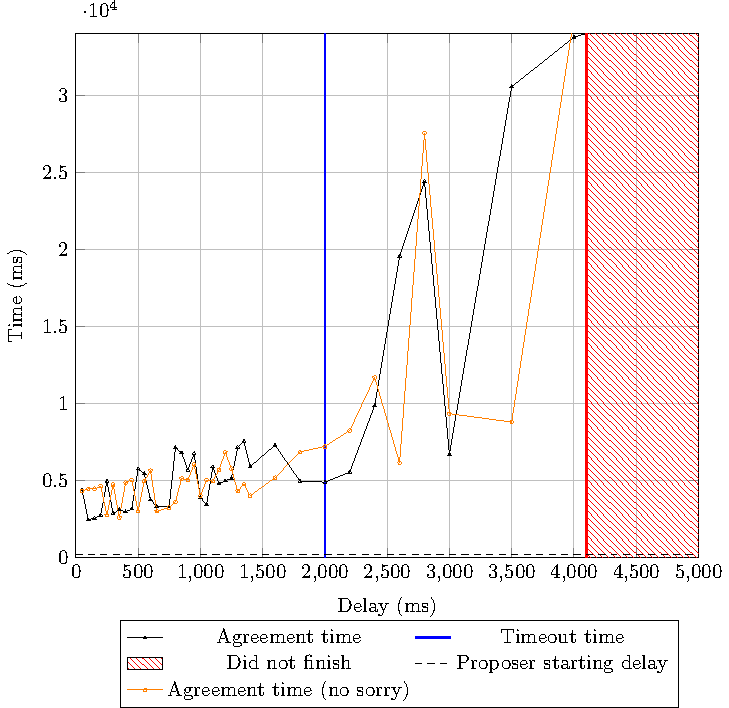
\includegraphics[width=\linewidth]{plots/nosorry.pdf}
    %\caption{Number of rounds needed to reach consensus respect to the delay $\text{proposer timeout}=2000$}
    \caption{Agreement time effects caused by removing sorry messages}
    \label{nosorry1}
\end{figure} 
The first experiment we tried was just commenting the whole sorry message thing, and the results obtained are shown at Figure \ref{nosorry1}. They were somewhat surprising as they don't paint a clear picture. We couldn't construct a satisfactory explanation, but then we remembered something: \textbf{we're using random numbers!} Noticing this, the solution is evident: uncomment the \textit{rand:uniform} calls.

\begin{figure}[H]
  \centering
  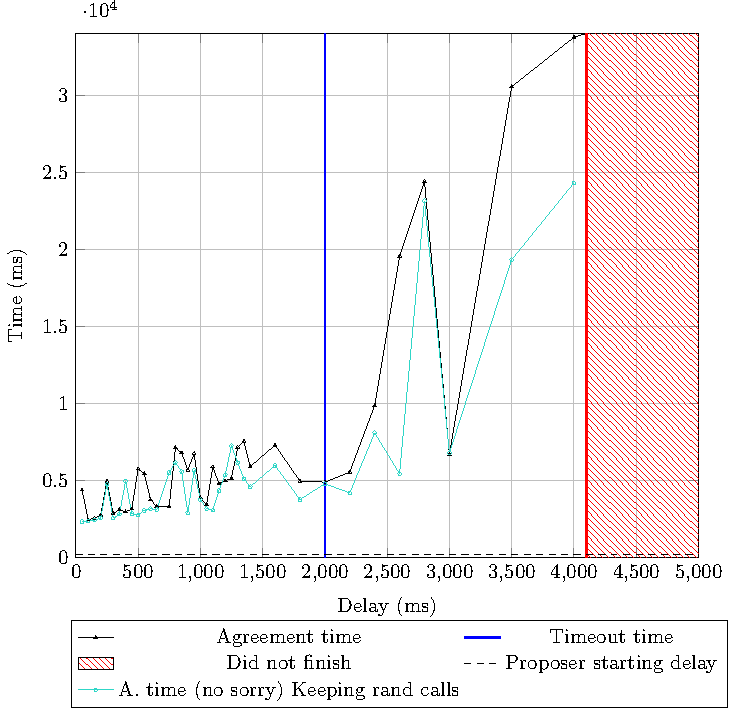
\includegraphics[width=\linewidth]{plots/nosorry2.pdf}
    %\caption{Number of rounds needed to reach consensus respect to the delay $\text{proposer timeout}=2000$}
    \caption{Removing sorry messages but keeping rand calls}
\end{figure} 

We rerun the experiments and got other results that are self-consistent over the range of delays considered on our test runs. We see that removing sorry message does in fact bring a bit of speedup. It is reasonable at we're not using this sorry messages for anything\footnote{At this point we're not using the improvement based on sorry messages. See Section \ref{sec:improvement}}.


%\subsubsection{Could you come to an agreement when sorry messages are not sent?}

\clearpage

\subsection{Try randomly dropping promise and vote messages in the acceptor}
\todo[inline]{Razonar por qué el algoritmo no falla en ningún caso}

We have studied the effects of dropping vote messages, promise messages and both at the same
time.

\begin{figure}[H]
  \centering
  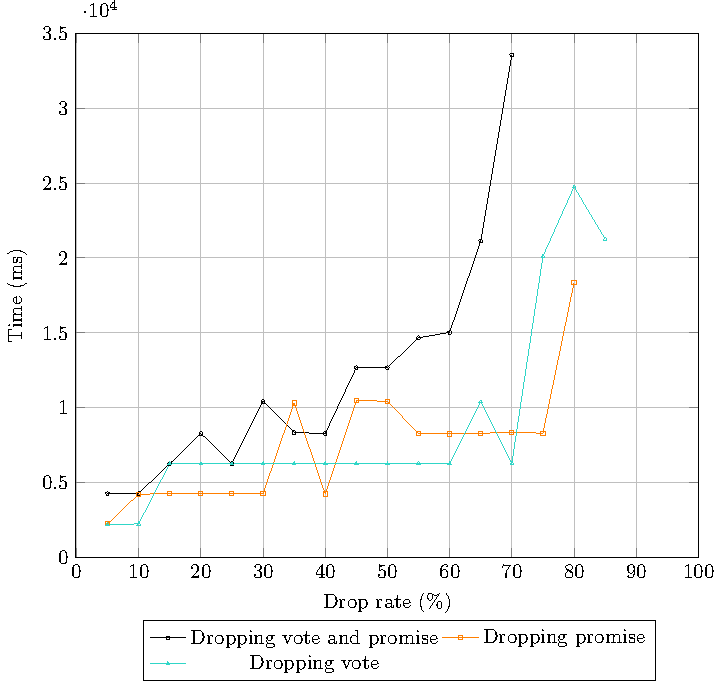
\includegraphics[width=\linewidth]{plots/dropboth.pdf}
    \caption{Agreement time w.r.t the drop ratio of both vote and promise messages}
\end{figure} 

Dropping a specific kind of message affects the agreement time significantly but isn't too
problematic unless we go to very high probabilities. Dropping both kinds of messages is obviously worse and specially so in the high end of the probability range.

Overall the algorithm seems pretty robust at first sight, because we're able to terminate even with very high dropping probabilities. Further tests with varying number of proposers/acceptors is due to reach strong conclusions but the results are encouraging.


\subsubsection{How does the drop ratio affect the number of rounds required to reach consensus?}
\begin{figure}[H]
  \centering
  \includegraphics[width=\linewidth]{plots/roundsdrop.pdf}
    \caption{Rounds w.r.t the drop ratio of both vote and promise messages}
\end{figure} 

The number of rounds is almost identical to the agreement time one.


\clearpage
\subsection{Try increasing the number of acceptors and proposers}

We have varied the number of proposers from $1$ to $8$ and the number of acceptors
from $1$ to $19$. Intuitively, the expected outcome is that adding proposers increases the number of conflicts and increases the agreement time. Adding acceptors should also impact the runtime negatively but much less noticeably. 

Of course they would also provide the system with resilience to problems that we have already considered such as message delays and message dropping under realistic circumstances. \todo[inline]{Check with jordi. Perhaps they add resilience when adverse conditions have $<$ 50\% probability but worsen the result otherwise??}



\begin{figure}[H]
  \centering
  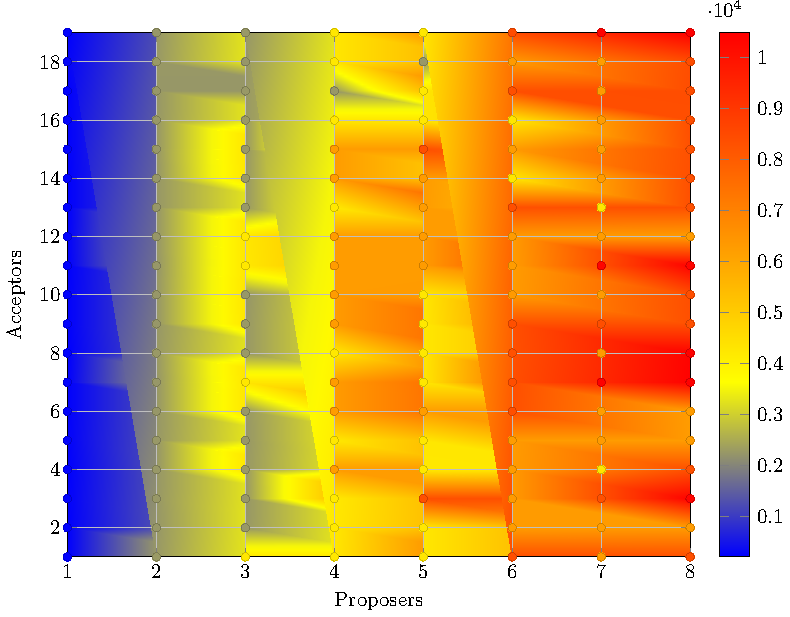
\includegraphics[width=\linewidth]{plots/exp4.pdf}
    \caption{Agreement time variation w.r.t nº of proposers and acceptors}
\end{figure} 

As there are meassurements present noise the surface plot is not too illuminating, thus we also present a 2D plot that we believe provides good insight in a clearer manner.

\begin{figure}[H]
  \centering
  \includegraphics[width=\linewidth]{plots/exp4_surf.pdf}
    \caption{Surface plot of agreement time variation w.r.t nº of proposers and acceptors}
\end{figure} 

Ignoring runtime spikes of unknown origin that might be caused by specific conditions of the testing system the results indicate what we expected. Increasing the number of proposers increases conflict and overall runtime. The effect of increasing acceptors is not so apparent, or at least it isn't in our testing results.



%\subsubsection{What is the impact of having more acceptors while keeping the number of proposers?}

\subsection{Adapt the paxy module to create the proposers and acceptors in a remote Erlang instance}



\section{Fault tolerance}

\subsection{Experiments}

\clearpage
\section{Improvement based on sorry messages}
\label{sec:improvement}

The improvement is fairly straightforward. We just have to mimic the procedure applied to the votes and promises for the sorry messages. Then, instead of timing out we can abort early when we're sure our proposal is not getting enough support to proceed with the voting phase.

\begin{figure}[H]
  \centering
  \includegraphics[width=\linewidth]{plots/improvement.pdf}
    \caption{Agreement time comparison between initial version, no sorry version and the improved version}
\end{figure} 

We have evaluated the effects with respect to the message delays, building on the work done at Subsections \ref{sec:delays} and \ref{sec:avoidsorry}. Results show that this improvement has a big impact for small delays, which should be the default scenario. When going past the timeout time at some points the improved version performs noticeably worse than the default.

\section{Personal opinion}

\textit{Provide your personal opinion of the seminar, indicating whether it should be included in next year's course or not.}

\end{document}
